\newpage
\lecture{5}{Способ приближения для особых матриц.}

В прошлой лекции был рассмотрен алгоритм вычисления сингулярного разложения, придуманный Голубом и Каханом.
Там же были описаны недостатки данного алгоритма, один из которых~--- отсутствие использования каких-либо свойств матрицы.

В данной лекции будут рассматриваться способ вычисления приближения в предположении, что матрица имеет некие свойства.

\subsection{Приближение матрицей малого ранга.}

Пусть матрицу $A$ размера $n\times n$ можно приблизить матрицей малого ранга $B$ ($\rk(B) = r \ll n$). Задача в поиске матрицы $B$.
Более того можно усложнить задачу. Пусть матрица изначальна дана не как $n^2$ своих элементов, а как некая дискретная функция от
двух аргументов: $a(i,\, j) = a_{ij}$. В реальности часто так и бывает~--- матрицы слишком большие, чтобы была физическая возможность
сохранить/передать все элементы матрицы, в то время как такая функция может быть довольно компактной (в терминах потребляемой при
вычислении памяти).

Итак, есть \textit{априорная} информация, то есть $A$ приближается матрицей $B$, которую в свою очередь можно записать
как
\[
    B = UV^T=\vect{u}_1\vect{v}_1^T+\ldots+\vect{u}_r\vect{v}_r^T, \quad U = [\vect{u}_1,\,\ldots,\, \vect{u}_r],\,
    V = [\vect{v}_1,\,\ldots,\, \vect{v}_r].
\]
Именно в таком виде и будем искать матрицу $B$, то есть в виде сомножителей.

\subsubsection{А реально ли..?}

\begin{wrapfigure}{r}{0.35\textwidth}
    \centering
    

\tikzset{every picture/.style={line width=0.75pt}} %set default line width to 0.75pt        

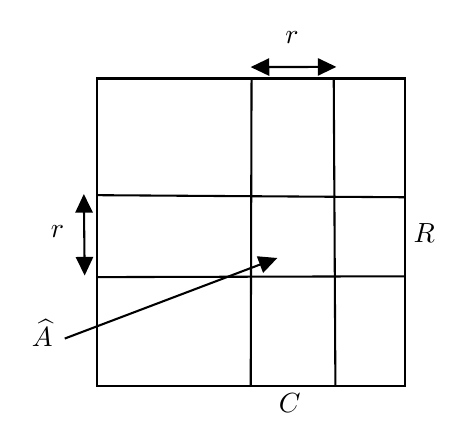
\begin{tikzpicture}[x=0.75pt,y=0.75pt,yscale=-1,xscale=1]
    %uncomment if require: \path (0,204); %set diagram left start at 0, and has height of 204

    %Shape: Square [id:dp18179701274889815] 
    \draw   (44.66,23.98) -- (192.86,23.98) -- (192.86,172.18) -- (44.66,172.18) -- cycle ;
    %Straight Lines [id:da34680283905684384] 
    \draw    (118.96,24.48) -- (118.56,171.68) ;
    %Straight Lines [id:da8821431178716612] 
    \draw    (158.56,24.08) -- (159.36,171.68) ;
    %Straight Lines [id:da45509046693738986] 
    \draw    (44.16,119.68) -- (192.96,119.28) ;
    %Straight Lines [id:da4329233968182751] 
    \draw    (44.6,80.2) -- (192.6,81.2) ;
    %Straight Lines [id:da2661200518992317] 
    \draw    (28.96,149.28) -- (128.55,111.54) ;
    \draw [shift={(131.36,110.48)}, rotate = 519.25] [fill={rgb, 255:red, 0; green, 0; blue, 0 }  ][line width=0.08]  [draw opacity=0] (8.93,-4.29) -- (0,0) -- (8.93,4.29) -- cycle    ;
    %Straight Lines [id:da8288824784988535] 
    \draw    (121.56,18.47) -- (156.8,18.41) ;
    \draw [shift={(159.8,18.4)}, rotate = 539.89] [fill={rgb, 255:red, 0; green, 0; blue, 0 }  ][line width=0.08]  [draw opacity=0] (8.93,-4.29) -- (0,0) -- (8.93,4.29) -- cycle    ;
    \draw [shift={(118.56,18.48)}, rotate = 359.89] [fill={rgb, 255:red, 0; green, 0; blue, 0 }  ][line width=0.08]  [draw opacity=0] (8.93,-4.29) -- (0,0) -- (8.93,4.29) -- cycle    ;
    %Straight Lines [id:da12627862047865435] 
    \draw    (38.19,82.68) -- (38.53,115.88) ;
    \draw [shift={(38.56,118.88)}, rotate = 269.42] [fill={rgb, 255:red, 0; green, 0; blue, 0 }  ][line width=0.08]  [draw opacity=0] (8.93,-4.29) -- (0,0) -- (8.93,4.29) -- cycle    ;
    \draw [shift={(38.16,79.68)}, rotate = 89.42] [fill={rgb, 255:red, 0; green, 0; blue, 0 }  ][line width=0.08]  [draw opacity=0] (8.93,-4.29) -- (0,0) -- (8.93,4.29) -- cycle    ;

    % Text Node
    \draw (195.6,92.6) node [anchor=north west][inner sep=0.75pt]   [align=left] {$\displaystyle R$};
    % Text Node
    \draw (130.6,174.2) node [anchor=north west][inner sep=0.75pt]   [align=left] {$\displaystyle C$};
    % Text Node
    \draw (11.6,138.6) node [anchor=north west][inner sep=0.75pt]   [align=left] {$\displaystyle \widehat{A}$};
    % Text Node
    \draw (133.8,0.00) node [anchor=north west][inner sep=0.75pt]   [align=left] {$\displaystyle r$};
    % Text Node
    \draw (20.8,93.58) node [anchor=north west][inner sep=0.75pt]   [align=left] {$\displaystyle r$};

\end{tikzpicture}
    \caption{Матрица $A$ ($\rk(A)=r$).}
    \label{fig:lect05_matrix}
\end{wrapfigure}

Сразу возникает закономерный вопрос: \textit{возможно ли без вычисления \textbf{всех} элементов матрицы найти её приближение?}

Рассмотрим частный граничный случай. Пусть $\rk(A)=r$. Тогда существуют $r$ столбцов и $r$ строк такие, что
\[
    A = C \widehat{A}^{-1}R,
\]
где $C,\, R,\, \widehat{A}$ смотри на рисунке \ref{fig:lect05_matrix} (на рисунке строки и столбцы не обязательно расположены
последовательно). Будем также называть существование таких строк и столбцов, как \mdef{существует крест}.

\begin{remark}
    $\widehat{A}$~--- невырожденная.
\end{remark}

Итак, если найти крест мы найдем и решение поставленной задачи.

А что если $\rk(A)\neq r$? Этот вопрос сложный по нескольким причинам. Во-первых, даже если такая матрица $\widehat{A}$ есть, и она невырожденная,
в ней могут быть слишком большие элементы, а вспоминая прошлые лекции, это сильно сказывается на точности вычислений. Соответственно,
вопрос еще сильнее усложняется: \textit{можно ли получить приближение приемлимой точности?} Ответом на вопрос служит довольно молодая теорема, которая представлена ниже,
но сначала введем важное понятие:

\begin{definition}
    \mdef{Объемом} квадратной матрицы назовем модуль её определителя.
\end{definition}

\begin{remark}
    Определение довольно естественное если вспомнить, что
    объем параллелепипеда, натянутого на столбцы (строки) матрицы и есть модуль ее определителя.
\end{remark}

\begin{theorem}[Гореинов--Тыртышников, 2000 г.]
    Пусть матрица $A$ имеет блочный вид:
    \[
        A = \left[
            \begin{array}{c|c}
                A_{11} & A_{12} \\
                \hline
                A_{21} & A_{22}
            \end{array}
            \right],\quad \begin{array}{l}
            A_{11}\text{~--- матрица } r\times r, \\
            A_{11}\text{~--- блок максимального объема среди всех } r\times r\text{"=блоков } A.
        \end{array}
    \]
    Пусть также
    \[
        \sigma_1\geqslant \sigma_2\geqslant\ldots\geqslant\sigma_r\geqslant\sigma_{r+1}\geqslant\ldots\text{~--- сингулярные числа матрицы $A$.}
    \]

    Тогда
    \[
        \left\| A - \left[
            \begin{array}{c}
                A_{11} \\
                A_{21}
            \end{array}
            \right]\cdot A_{11}^{-1}\cdot \left[
            \begin{array}{cc}
                A_{11} & A_{12}
            \end{array}
            \right]\right\|_{C}\leqslant (r+1)\sigma_{r+1},
    \]
    где $\|A\|_C:=\max\limits_{i,\,j} |a_{ij}|$.

    \begin{proof}
        Распишем матрицу под знаком нормы:
        \begin{align*}
            \left[
                \begin{array}{cc}
                    A_{11} & A_{12} \\
                    A_{21} & A_{22}
                \end{array}
                \right]-\left[
                \begin{array}{c}
                    A_{11} \\
                    A_{21}
                \end{array}
                \right]\cdot A_{11}^{-1}\cdot \left[
                \begin{array}{cc}
                    A_{11} & A_{12}
                \end{array}
            \right] & =\left[
                \begin{array}{cc}
                    A_{11} & A_{12} \\
                    A_{21} & A_{22}
                \end{array}
                \right]-\left[
                \begin{array}{cc}
                    A_{11} & A_{12}                  \\
                    A_{21} & A_{21}A_{11}^{-1}A_{12}
                \end{array}
                \right]=      \\
                    & =\left[
                \begin{array}{cc}
                    0 & 0 \\
                    0 & H
                \end{array}
                \right], \quad \text{где }H = A_{22}-A_{21}A_{11}^{-1}A_{12}.
        \end{align*}

        \begin{remark}
            Матрица $H$ также называется \mdef{дополнением по Шуру} блока $A_{11}$ в матрице $A$.
        \end{remark}

        Нужно оценить максимальных элемент в матрице $H$. Рассмотрим элемент $\alpha$ в позиции $(i,\,j)$.
        Формулу выше можно написать для этого элемента таким образом: пусть $\vect{v}$~--- $i$"=ая строка,
        $\vect{u}$~--- $j$"=ый столбец, тогда:

        \[
            \underbrace{\left[
                    \begin{array}{cc}
                        A_{11}     & \vect{u} \\
                        \vect{v}^T & \alpha
                    \end{array}
                    \right]}_{\widetilde{A}} - \left[
                \begin{array}{c}
                    A_{11} \\
                    \vect{v}^T
                \end{array}
                \right]\cdot A_{11}^{-1}\cdot\left[
                \begin{array}{cc}
                    A_{11} & \vect{u}
                \end{array}
                \right] = \left[
                \begin{array}{cc}
                    0 & 0 \\
                    0 & h
                \end{array}
                \right], \quad h = \alpha - \vect{v}^TA_{11}^{-1}\vect{u}.
        \]

        Для оценки элемента $h$ нужно воспользоваться тем, что матрица $A_{11}$ имеет \textbf{наибольший} объем среди любых
        $r\times r$ подматриц. Проведем один шаг блочного исключения~--- обнулим $\vect{v}^T$:
        \[
            \underbrace{\left[
                    \begin{array}{cc}
                        I                      & 0 \\
                        -\vect{v}^TA_{11}^{-1} & 1
                    \end{array}
                    \right]}_{M}\cdot
            \left[
                \begin{array}{cc}
                    A_{11}     & \vect{u} \\
                    \vect{v}^T & \alpha
                \end{array}
                \right] = \left[
                \begin{array}{cc}
                    A_{11} & \vect{u} \\
                    0      & h
                \end{array}
                \right]
            \label{eq:delet}
        \]
        Теперь перейдем к обратным матрицам:
        \[
            \left[
                \begin{array}{cc}
                    A_{11}     & \vect{u} \\
                    \vect{v}^T & \alpha
                \end{array}
                \right]^{-1}\cdot\underbrace{\left[
                    \begin{array}{cc}
                        I                & 0 \\
                        \vect{v}^TA_{11} & 1
                    \end{array}
                    \right]}_{M^{-1}}=\left[
                \begin{array}{cc}
                    A_{11}^{-1} & -A_{11}^{-1}\vect{u}h^{-1} \\
                    0           & h^{-1}
                \end{array}
                \right]
        \]
        Далее умножим обе части справа на $M$:
        \[
            \left[
                \begin{array}{cc}
                    A_{11}     & \vect{u} \\
                    \vect{v}^T & \alpha
                \end{array}
                \right]^{-1}=\left[
                \begin{array}{cc}
                    A_{11}^{-1} & -A_{11}^{-1}\vect{u}h^{-1} \\
                    0           & h^{-1}
                \end{array}
                \right]\cdot \left[
                \begin{array}{cc}
                    I                      & 0 \\
                    -\vect{v}^TA_{11}^{-1} & 1
                \end{array}
                \right]=\left[
                \begin{array}{cc}
                    * & *      \\
                    * & h^{-1}
                \end{array}
                \right]
        \]

        Заметим, что $h^{-1}$~--- это элемент матрицы $\widetilde{A}^{-1}$ (определение $\widetilde{A}$ смотри выше) в правом нижнем углу.
        Рассмотрим определитель матрицы $\widetilde{A}$:
        \[
            |\widetilde{A}|=|A_{11}|\cdot |h|.
        \]
        Итак, если матрица $A_{11}$ имеет максимальный объем в $\widetilde{A}$, тогда $h^{-1}$~--- максимальный
        по модулю элемент матрицы $\widetilde{A}^{-1}$.

        Теперь рассмотрим сингулярную норму матрицы $\widetilde{A}^{-1}$:
        \[
            \|\widetilde{A}^{-1}\|_2=\sigma_{\max}(\widetilde{A}^{-1})\leqslant \|\widetilde{A}^{-1}\|_{F} =
            \sqrt{\sum_{i,\, j} |(\widetilde{A}^{-1})_{ij}|^2}\leqslant (r+1)|h^{-1}|
        \]

        Откуда получаем, что
        \[
            |h|\leqslant\dfrac{r+1}{\sigma_{\max}\left(\widetilde{A}^{-1}\right)}.
        \]

        Далее воспользуемся следующим утверждением (доказательство смотри в \nameref{sect:con})
        \begin{claim}
            Если $\widetilde{\sigma}_1\geqslant\ldots\geqslant\widetilde{\sigma}_r\geqslant\widetilde{\sigma}_{r+1}$~--- сингулярные числа
            матрицы $\widetilde{A}$, то сингулярные числа матрицы $\widetilde{A}^{-1}$~--- это
            $\widetilde{\sigma}^{-1}_1\leqslant\ldots\leqslant\widetilde{\sigma}^{-1}_{r+1}$.
        \end{claim}

        Итак,
        \[
            |h|\leqslant\dfrac{r+1}{\sigma_{\max}\left(\widetilde{A}^{-1}\right)}\leqslant(r +1)\cdot\sigma_{\min}(\widetilde{A}) =
            (r+1)\widetilde{\sigma}_{r+1}.
        \]

        Осталось понять почему $\widetilde{\sigma}_{r+1}\leqslant\sigma_{r+1}$. Здесь на помощь приходит важное утверждение:

        \begin{claim}[о соотношении разделения сингулярных чисел]
            Для матрицы $A$ и её подматрицы $\widetilde{A}$ порядка $k$ верно, что $\sigma_k(\widetilde{A})\leqslant\sigma_k(A)$.
        \end{claim}

    \end{proof}
\end{theorem}

\subsection{Немного об эрмитовых матрицах.}

Рассмотрим эрмитовую матрицу $A\in\Cx^{n\times n}$, то есть $A=A^*$. Занумеруем её собственные значения в порядке невозрастания:
$\lambda_{1}(A)\geqslant\ldots\geqslant\lambda_n(A)$. Справедлива следующая теорема (вариационная характеризация собственных значений):

\begin{theorem}[Куранта--Фишера]
    \[
        \lambda_k(A) = \max_{L_k}\min_{\substack{\vect{x}\in L_k\\ \vect{x}\neq 0}}
        \underbrace{\dfrac{(A\vect{x},\, \vect{x})}{(\vect{x},\,\vect{x})}}_{\substack{\text{отношение}\\\text{Рэлея}}},
    \]
    где $L_k$~--- пространство размерности $k$.
\end{theorem}

Еще существует так называемый закон инерции для эрмитовых матриц:

\begin{theorem}[закон инерции]
    Пусть $\nu_{+},\,\nu_{-},\,\nu_{0}$~--- число положительных, отрицательных и нулевых собственных значений соответственно.
    Тогда эта тройка сохраняется для конгруэнтных матриц:
    \[
        (\nu_{+},\, \nu_{-},\, \nu_{0})(A) = (\nu_{+},\, \nu_{-},\, \nu_{0})(P^*AP), \quad\forall\text{ невыржденной } P.
    \]
\end{theorem}

Можно доказать, что последние две теоремы эквивалентны (одна выводится из другой и наоборот). Более того существует еще
один факт, который эквивалентен этим двум.
\newpage

\begin{theorem}[соотношение разделения]
    Пусть матрица $A$~--- эрмитова. Пусть $B$~--- её подматрица порядка на 1 меньше. Тогда
    \[
        \lambda_1(A)\geqslant\lambda_1(B)\geqslant\lambda_2(A)\geqslant\lambda_2(B)\geqslant\ldots
    \]
\end{theorem}

\subsection{Связи сингулярных чисел.}
\label{sect:con}

Поставим такую задачу. Как связаны сингулярные числа матриц $A$ и $B=[A,\vect{u}]$?

Во-первых, $\sigma_i^2(A)$~--- собственные числа матрицы $A^*A$~--- эрмитова. Аналогично, если рассмотреть расширенную матрицу:
\[
    \left[
        \begin{array}{cc}
            A & \vect{u}
        \end{array}
        \right]^*\cdot\left[
        \begin{array}{cc}
            A & \vect{u}
        \end{array}
        \right]=\left[
        \begin{array}{c}
            A^* \\
            u^*
        \end{array}
        \right]\cdot\left[
        \begin{array}{cc}
            a & \vect{u}
        \end{array}
        \right] = \left[
        \begin{array}{c|c}
            A^*A        & A^*\vect{u}        \\
            \hline
            \vect{u}^*A & \vect{u}^*\vect{u}
        \end{array}
        \right].
\]
Откуда из соотношения разделения получаем, что $\sigma_k^2(B)\geqslant\sigma_k^2(A)$.

\subsection{Ещё один алгоритм...}

Еще не было оговорено, а как найти подматрицу наибольшего объема? Здесь поможет следующий алгоритм.

\begin{figure}[!ht]
    \centering
    \begin{minipage}{.5\textwidth}
        \centering
        \tikzset{every picture/.style={line width=0.75pt}} %set default line width to 0.75pt        

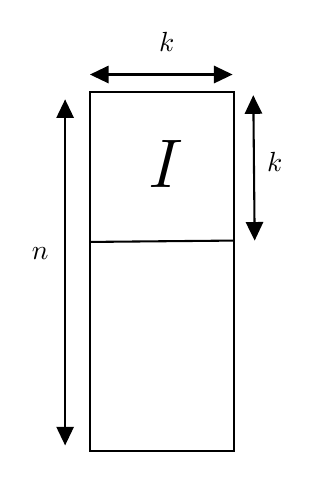
\begin{tikzpicture}[x=0.75pt,y=0.75pt,yscale=-1,xscale=1]
%uncomment if require: \path (0,300); %set diagram left start at 0, and has height of 300

%Shape: Rectangle [id:dp4540860363039436] 
\draw   (50.87,88.67) -- (120.2,88.67) -- (120.2,261.4) -- (50.87,261.4) -- cycle ;
%Straight Lines [id:da3693463850785983] 
\draw    (38.87,95.07) -- (38.87,255.73) ;
\draw [shift={(38.87,258.73)}, rotate = 270] [fill={rgb, 255:red, 0; green, 0; blue, 0 }  ][line width=0.08]  [draw opacity=0] (8.93,-4.29) -- (0,0) -- (8.93,4.29) -- cycle    ;
\draw [shift={(38.87,92.07)}, rotate = 90] [fill={rgb, 255:red, 0; green, 0; blue, 0 }  ][line width=0.08]  [draw opacity=0] (8.93,-4.29) -- (0,0) -- (8.93,4.29) -- cycle    ;
%Straight Lines [id:da0034688381143717084] 
\draw    (53.87,80.07) -- (116.53,80.07) ;
\draw [shift={(119.53,80.07)}, rotate = 180] [fill={rgb, 255:red, 0; green, 0; blue, 0 }  ][line width=0.08]  [draw opacity=0] (8.93,-4.29) -- (0,0) -- (8.93,4.29) -- cycle    ;
\draw [shift={(50.87,80.07)}, rotate = 0] [fill={rgb, 255:red, 0; green, 0; blue, 0 }  ][line width=0.08]  [draw opacity=0] (8.93,-4.29) -- (0,0) -- (8.93,4.29) -- cycle    ;
%Straight Lines [id:da9300394535026744] 
\draw    (50.87,160.73) -- (120.2,160.07) ;
%Straight Lines [id:da18772043066774846] 
\draw    (129.56,93.07) -- (130.17,157.07) ;
\draw [shift={(130.2,160.07)}, rotate = 269.45] [fill={rgb, 255:red, 0; green, 0; blue, 0 }  ][line width=0.08]  [draw opacity=0] (8.93,-4.29) -- (0,0) -- (8.93,4.29) -- cycle    ;
\draw [shift={(129.53,90.07)}, rotate = 89.45] [fill={rgb, 255:red, 0; green, 0; blue, 0 }  ][line width=0.08]  [draw opacity=0] (8.93,-4.29) -- (0,0) -- (8.93,4.29) -- cycle    ;

% Text Node
\draw (21.33,162) node [anchor=north west][inner sep=0.75pt]   [align=left] {$\displaystyle n$};
% Text Node
\draw (82.67,58) node [anchor=north west][inner sep=0.75pt]   [align=left] {$\displaystyle k$};
% Text Node
\draw (134.67,116) node [anchor=north west][inner sep=0.75pt]   [align=left] {$\displaystyle k$};
% Text Node
\draw (77.33,110.33) node [anchor=north west][inner sep=0.75pt]  [font=\Huge] [align=left] {$\displaystyle I$};


\end{tikzpicture}

        \caption{Итог шага \protect\circled{1}.}
        \label{fig:lect05_algo}
    \end{minipage}%
    \begin{minipage}{.5\textwidth}
        \centering
        

\tikzset{every picture/.style={line width=0.75pt}} %set default line width to 0.75pt        

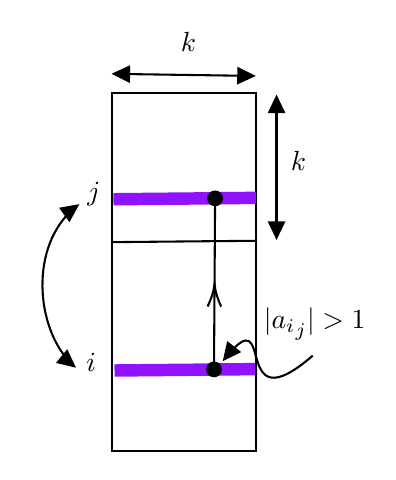
\begin{tikzpicture}[x=0.75pt,y=0.75pt,yscale=-1,xscale=1]
%uncomment if require: \path (0,300); %set diagram left start at 0, and has height of 300

%Straight Lines [id:da3987772168380741] 
\draw [color={rgb, 255:red, 144; green, 19; blue, 254 }  ,draw opacity=1 ][fill={rgb, 255:red, 245; green, 166; blue, 35 }  ,fill opacity=1 ][line width=2.25]    (52.02,221.07) -- (120.69,220.4)(52.05,224.07) -- (120.71,223.4) ;
%Shape: Rectangle [id:dp4540860363039436] 
\draw   (50.87,88.67) -- (120.2,88.67) -- (120.2,261.4) -- (50.87,261.4) -- cycle ;
%Straight Lines [id:da9300394535026744] 
\draw    (50.87,160.73) -- (120.2,160.07) ;
%Shape: Circle [id:dp49882419469536754] 
\draw  [fill={rgb, 255:red, 0; green, 0; blue, 0 }  ,fill opacity=1 ] (96.67,222.03) .. controls (96.67,220.21) and (98.14,218.73) .. (99.97,218.73) .. controls (101.79,218.73) and (103.27,220.21) .. (103.27,222.03) .. controls (103.27,223.86) and (101.79,225.33) .. (99.97,225.33) .. controls (98.14,225.33) and (96.67,223.86) .. (96.67,222.03) -- cycle ;
%Curve Lines [id:da6941956227421298] 
\draw    (147.53,215.4) .. controls (107.68,250.03) and (129.93,186.69) .. (105.74,216.15) ;
\draw [shift={(104.2,218.07)}, rotate = 308.11] [fill={rgb, 255:red, 0; green, 0; blue, 0 }  ][line width=0.08]  [draw opacity=0] (8.93,-4.29) -- (0,0) -- (8.93,4.29) -- cycle    ;
%Straight Lines [id:da581564015532243] 
\draw [color={rgb, 255:red, 144; green, 19; blue, 254 }  ,draw opacity=1 ][fill={rgb, 255:red, 245; green, 166; blue, 35 }  ,fill opacity=1 ][line width=2.25]    (51.52,138.57) -- (120.19,137.9)(51.55,141.57) -- (120.21,140.9) ;
%Curve Lines [id:da6167939978320494] 
\draw    (31.2,219.19) .. controls (14.1,202.25) and (10.7,162.58) .. (32.94,144.09) ;
\draw [shift={(35.08,142.44)}, rotate = 504.29] [fill={rgb, 255:red, 0; green, 0; blue, 0 }  ][line width=0.08]  [draw opacity=0] (8.93,-4.29) -- (0,0) -- (8.93,4.29) -- cycle    ;
\draw [shift={(33.48,221.24)}, rotate = 219.23] [fill={rgb, 255:red, 0; green, 0; blue, 0 }  ][line width=0.08]  [draw opacity=0] (8.93,-4.29) -- (0,0) -- (8.93,4.29) -- cycle    ;
%Straight Lines [id:da21720808633398558] 
\draw    (53.6,79.69) -- (117.1,80.61) ;
\draw [shift={(120.1,80.65)}, rotate = 180.82] [fill={rgb, 255:red, 0; green, 0; blue, 0 }  ][line width=0.08]  [draw opacity=0] (8.93,-4.29) -- (0,0) -- (8.93,4.29) -- cycle    ;
\draw [shift={(50.6,79.65)}, rotate = 0.82] [fill={rgb, 255:red, 0; green, 0; blue, 0 }  ][line width=0.08]  [draw opacity=0] (8.93,-4.29) -- (0,0) -- (8.93,4.29) -- cycle    ;
%Straight Lines [id:da2305583187553364] 
\draw    (130.1,92.65) -- (130.1,156.65) ;
\draw [shift={(130.1,159.65)}, rotate = 270] [fill={rgb, 255:red, 0; green, 0; blue, 0 }  ][line width=0.08]  [draw opacity=0] (8.93,-4.29) -- (0,0) -- (8.93,4.29) -- cycle    ;
\draw [shift={(130.1,89.65)}, rotate = 90] [fill={rgb, 255:red, 0; green, 0; blue, 0 }  ][line width=0.08]  [draw opacity=0] (8.93,-4.29) -- (0,0) -- (8.93,4.29) -- cycle    ;
%Straight Lines [id:da3001798860066407] 
\draw [line width=0.75]    (100.5,139.65) -- (99.97,222.03) ;
\draw [shift={(100.23,180.84)}, rotate = 90.37] [color={rgb, 255:red, 0; green, 0; blue, 0 }  ][line width=0.75]    (10.93,-3.29) .. controls (6.95,-1.4) and (3.31,-0.3) .. (0,0) .. controls (3.31,0.3) and (6.95,1.4) .. (10.93,3.29)   ;
%Shape: Circle [id:dp025947933375819465] 
\draw  [fill={rgb, 255:red, 0; green, 0; blue, 0 }  ,fill opacity=1 ] (97.2,139.65) .. controls (97.2,137.83) and (98.68,136.35) .. (100.5,136.35) .. controls (102.32,136.35) and (103.8,137.83) .. (103.8,139.65) .. controls (103.8,141.47) and (102.32,142.95) .. (100.5,142.95) .. controls (98.68,142.95) and (97.2,141.47) .. (97.2,139.65) -- cycle ;

% Text Node
\draw (122.5,190.67) node [anchor=north west][inner sep=0.75pt]   [align=left] {$\displaystyle {|a_{i}}_{j} | >1$};
% Text Node
\draw (37.5,130.5) node [anchor=north west][inner sep=0.75pt]   [align=left] {$\displaystyle j$};
% Text Node
\draw (37,213) node [anchor=north west][inner sep=0.75pt]   [align=left] {$\displaystyle i$};
% Text Node
\draw (82.5,57.9) node [anchor=north west][inner sep=0.75pt]   [align=left] {$\displaystyle k$};
% Text Node
\draw (135.5,115.4) node [anchor=north west][inner sep=0.75pt]   [align=left] {$\displaystyle k$};


\end{tikzpicture}

        \caption{Итерация в шаге \protect\circled{2}.}
        \label{fig:lect05_step2}
    \end{minipage}
\end{figure}

Пусть матрица имеет <<стоячий>> вид (смотри рисунок \ref{fig:lect05_algo}).

\begin{enumerate}[label=\protect\circled{\arabic*}]
    \item Найдем в матрице невырожденную подматрицу $k\times k$ и переместим ее наверх. Далее умножим матрицу справа
          на обратную к найденной невырожденной, в итоге получится матрица, вид которой изображен на рисунке \ref{fig:lect05_algo}. Отметим также
          что умножение на невыржденную матрицу не изменяет отношения объема.
    \item Теперь в нижней части матрицы найдем наибольшее число $a_{ij}$. Допустим, оно оказалось по модулю больше 1\footnote{на самом деле 
    можно сравнивать не с 1, а с $1+\delta$, то есть искать не максимальный объем, но близкий к нему.} 
    (иначе алгоритм завершен). 
    Тогда поменяем местами строки $i$ и $j$. Тогда модуль определителя верхней подматрицы станет равным $|a_{ij}|$, то есть нашли подматрицу большего объема. 
    Остается вернутся к пункту \protect\circled{1} и выполнить шаги еще раз.
\end{enumerate}